\section{Results}

\setlength{\tabcolsep}{4pt} % default ~6pt

\begin{table}[!ht]
    \caption{Regression parameters for the light spring.}
    \centering
    \begin{tabular}{|
        S[table-format=1.5,table-number-alignment=center] !{\vrule width 1.2pt}
        S[table-format=1.6] |
        S[table-format=2.2] |
        S[table-format=1.4] !{\vrule width 1.2pt}
        S[table-format=2.4] |
        S[table-format=3.1] |
    }
    \hline
    \rowcolor{lightgray}
    {$m{\textsubscript{load}}$} & {$\gamma$} & {$\omega'$} & {$R^2$} & {${m{\textsubscript{load}}}^{-1}$} & {$\omega'^2 + \gamma^2$} \\
    \rowcolor{lightgray}
    {(\si{\kilo\gram})} & {(\si{\per\second})} & {(\si{\radian\per\second})} & {} & {(\si{\per\kilo\gram})} & {(\si{\per\second\squared})} \\
    \hline
    0.05025 & 0.024240 & 21.47 & 0.9990 & 19.90  & 461.0 \\
    0.10014 & 0.019520 & 15.43 & 0.8385 & 9.9860 & 238.1 \\
    0.15044 & 0.015780 & 12.53 & 0.9947 & 6.6472 & 157.0 \\
    0.20011 & 0.012860 & 10.89 & 0.9996 & 4.9973 & 118.6 \\
    0.25019 & 0.012236 & 9.75 & 0.9894 & 3.9970 & 95.1 \\
    0.30012 & 0.011830 & 8.92 & 0.9999 & 3.3320 & 79.5 \\
    0.34991 & 0.011380 & 8.28 & 0.9999 & 2.8579 & 68.6 \\
    \hline
    \end{tabular}
    \label{tab:lightspring}
\end{table}

\begin{table}[!ht]
    \caption{Regression parameters for the stiff spring.}
    \centering
    \begin{tabular}{|
        S[table-format=1.5,table-number-alignment=center] !{\vrule width 1.2pt}
        S[table-format=1.6] |
        S[table-format=2.2] |
        S[table-format=1.4] !{\vrule width 1.2pt}
        S[table-format=1.4] |
        S[table-format=3.1] |
    }
    \hline
    \rowcolor{lightgray}
    {$m{\textsubscript{load}}$} & {$\gamma$} & {$\omega'$} & {$R^2$} & {${m{\textsubscript{load}}}^{-1}$} & {$\omega'^2 + \gamma^2$} \\
    \rowcolor{lightgray}
    {(\si{\kilo\gram})} & {(\si{\per\second})} & {(\si{\radian\per\second})} & {} & {(\si{\per\kilo\gram})} & {(\si{\per\second\squared})} \\
    \hline
    0,30010 & 0,007771 & 13,41 & 0,9971 & 3,3322 & 179,8 \\
	0,35014 & 0,006539 & 12,45 & 0,9955 & 2,8560 & 155,0 \\
	0,40014 & 0,005946 & 11,67 & 0,9993 & 2,4991 & 136,2 \\
	0,45004 & 0,005352 & 11,02 & 0,9993 & 2,2220 & 121,4 \\
	0,49984 & 0,004909 & 10,47 & 0,9995 & 2,0006 & 109,6 \\
    \hline
    \end{tabular}
    \label{tab:stiffspring}
\end{table}

\begin{table}[!h]
	\caption{Regression parameters for two stiff springs in series.}
    \centering
    \begin{tabular}{|
        S[table-format=1.5,table-number-alignment=center] !{\vrule width 1.2pt}
        S[table-format=1.6] |
        S[table-format=2.2] |
        S[table-format=1.4] !{\vrule width 1.2pt}
        S[table-format=1.4] |
        S[table-format=3.1] |
    }
    \hline
    \rowcolor{lightgray}
    {$m{\textsubscript{load}}$} & {$\gamma$} & {$\omega'$} & {$R^2$} & {${m{\textsubscript{load}}}^{-1}$} & {$\omega'^2 + \gamma^2$} \\
    \rowcolor{lightgray}
    {(\si{\kilo\gram})} & {(\si{\per\second})} & {(\si{\radian\per\second})} & {} & {(\si{\per\kilo\gram})} & {(\si{\per\second\squared})} \\
    \hline
    0,30010 & 0,004957 & 9,581 & 0,9996 & 3,3322 & 91,80 \\
	0,35014 & 0,004321 & 8,907 & 0,9995 & 2,8560 & 79,33 \\
	0,40014 & 0,003469 & 8,363 & 0,9991 & 2,4991 & 69,94 \\
	0,45004 & 0,003112 & 7,907 & 0,9995 & 2,2220 & 62,52 \\
	0,49984 & 0,002791 & 7,517 & 0,9996 & 2,0006 & 56,51 \\
    \hline
    \end{tabular}
    \label{tab:seriesstiffsprings}
\end{table}

\clearpage
\onecolumn

\begin{graph}[H]
    \centering
    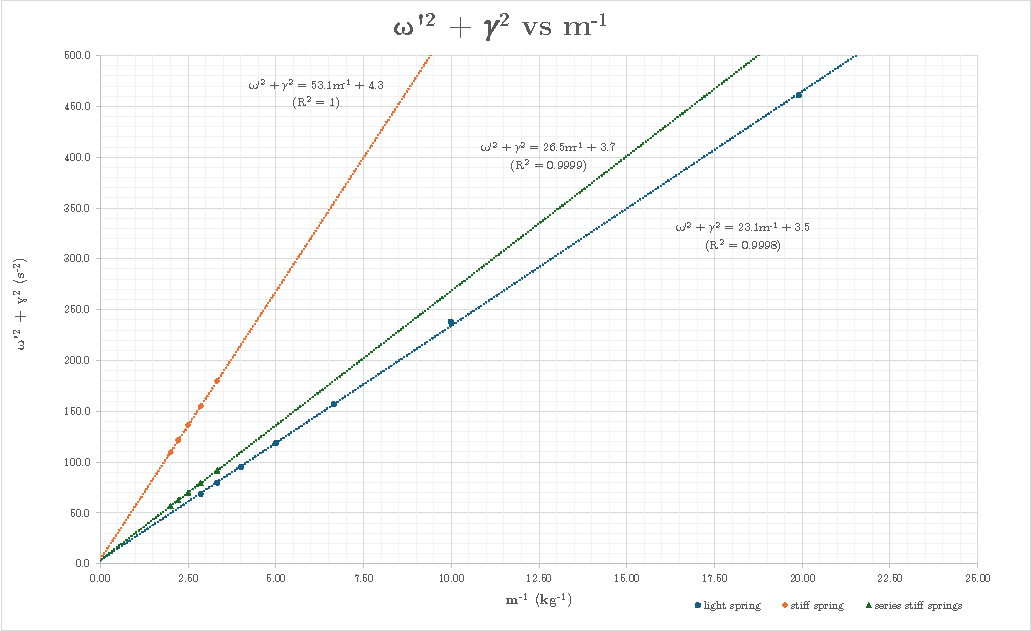
\includegraphics[width=1\textwidth]{images/graph1.pdf}
    \caption{Relationship between $\omega'^2 + \gamma^2$ and ${m{\textsubscript{load}}}^{-1}$ for different spring configurations, where the gradient represents the spring constant ($k$).}
\end{graph}

\begin{graph}[H]
    \centering
    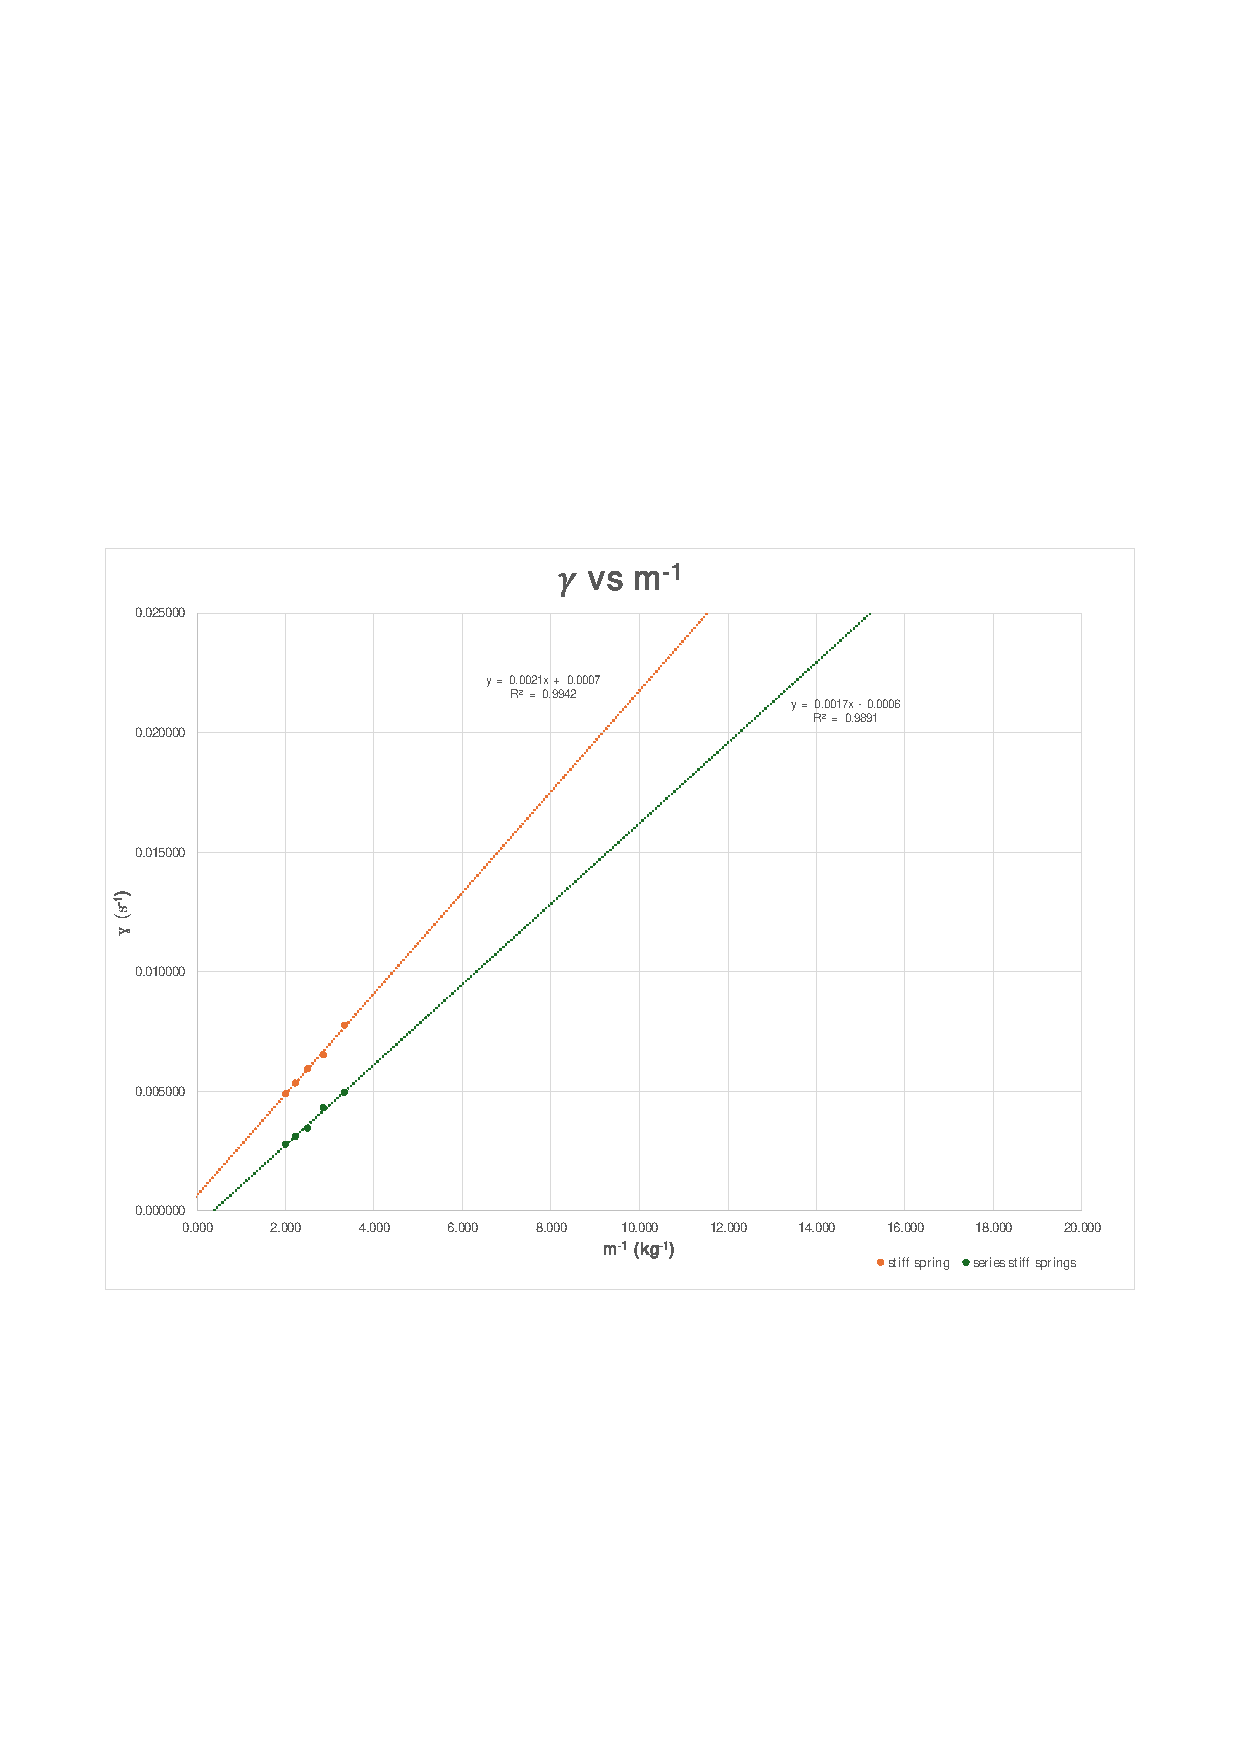
\includegraphics[width=1\textwidth]{images/graph2.pdf}
    \caption{Relationship between $\gamma$ and ${m{\textsubscript{load}}}^{-1}$ for different spring configurations, where the gradient represents half the damping coefficient ($\tfrac{b}{2}$).}
\end{graph}

\twocolumn

\begin{strip}
\vspace{-4em}
\begin{multicols}{2}
\noindent
\begin{align*}
\intertext{For $\textbf{Graph 1}$: $k = \text{gradient}$.}
k_{\text{light}} &= \frac{\Delta (\omega'^2 + \gamma^2)}{\Delta m_{\text{load}}^{-1}} \\
&= \frac{315.0 - 165.0}{13.50 - 7.00} \\
&= 23.1 \; \si{\kilo\gram\per\second\squared} \; \text{(3 s.f.)} \\[1em]
k_{\text{single stiff}} &= \frac{\Delta (\omega'^2 + \gamma^2)}{\Delta m_{\text{load}}^{-1}} \\
&= \frac{375.0 - 30.0}{7.00 - 0.50} \\
&= 53.1 \; \si{\kilo\gram\per\second\squared} \; \text{(3 s.f.)} \\[1em]
k_{\text{series series}} &= \frac{\Delta (\omega'^2 + \gamma^2)}{\Delta m_{\text{load}}^{-1}} \\
&= \frac{480.0 - 255.0}{18.00 - 9.50} \\
&= 26.5 \; \si{\kilo\gram\per\second\squared} \; \text{(3 s.f.)}
\end{align*}

\columnbreak

\noindent
\begin{align*}
\intertext{For $\textbf{Graph 2}$: $b = 2 \times \text{gradient}$.}
b_{\text{single stiff}} &= 2 \times \frac{\Delta \gamma}{\Delta m_{\text{load}}^{-1}} \\
&= 2 \times \frac{\left(9.375 - 4.688 \right) \times 10^{-3}}{4.12 - 1.90} \\
&= 4.22 \times 10^{-3} \; \si{\kilo\gram\per\second} \; \text{(3 s.f.)} \\[1em]
b_{\text{series stiff}} &= 2 \times \frac{\Delta (\omega'^2 + \gamma^2)}{\Delta m_{\text{load}}^{-1}} \\
&= 2 \times \frac{\left(6.875 - 1.250 \right) \times 10^{-3}}{4.40 - 1.10} \\
&= 3.40 \times 10^{-3} \; \si{\kilo\gram\per\second} \; \text{(3 s.f.)}
\end{align*}
\end{multicols}
\captionof{figure}{Calculations of $k$ and $b$ values from graphs.}
\end{strip}
\nopagebreak